\section{STM32F4}
La Board si divide in due settori: Uno che contiene l'interfaccia di programmazione (si tratta di una scheda di progettazione), e si tratta di un altro microcontrollore removibile della ST che fa da interfaccia verso il computer (riceve il binario dal pc, e si interfaccia con il core con protocollo SVG o JTAG); L'altro settore invece contiene il SoC, che è proprio l'oggetto etichettato STM32F407VTGT6 (fig \ref{img:STM32F4}), mentre tutto ciò che c'è intorno consente all'utente di interfacciarsi con il SoC. 
I piedini presenti tra il SoC e la board sono condivisi tra più periferiche, quindi in fase di configurazione dobbiamo capire quale delle periferiche lo userà. Questi \textit{piedini} poi dovranno interagire con il mondo esterno, e ci viene in aiuto il \textit{jumper cable} che consente di collegare i pin della board con la periferica esterna.


\begin{figure}[h!]
    \centering
    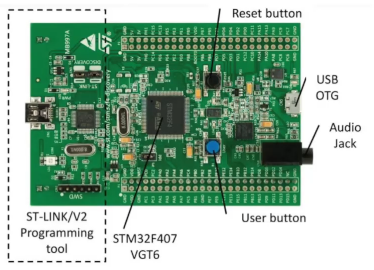
\includegraphics[width=.7\textwidth]{img/STM32F4.png}
    \caption{STM32F4}
    \label{img:STM32F4}
\end{figure}


Le periferiche illustrate sul \textit{reference manual} sono memory mapped, quindi raggiungibile mediante accessi in memoria. Per ogni periferica, in fase di configurazione si va a scrivere in alcuni registri in memoria. 

\subsection{CubeIDE}
L'IDE utilizzato al corso per la programmazione della scheda è STM32CubeIDE.
Selezionare la giusta board è importante perchè non si sta programmando un SoC nudo, ma una board, dove le periferiche sono mappate in maniera fissa su alcune piedinature del SoC. 
Una volta creato il progetto, ST fornisce un'interfaccia grafica per configurare i pin del MCU. 
Poichè i pin sono molto numerosi, sono raggruppati in \textit{porte}, enumerate con lettere. Ogni porta gestisce un determianto sottoinsieme di PIN. 
Onde evitare di configurare ogni periferica attraverso l'accesso in memoria e il modello di programmazione, i produttori di microcontrollori offrono un'astrazione delle periferiche denominate \textbf{HAL} (Hardware abstraction layer). Questi offrono un'interfaccia di programmazione astratta della periferica. 

\subsection{Gestione mutua esclusione}
Per parlare della necessità della mutua esclusione, conviene partire da un esempio.
Consideriamo la trasmissione UART in ISR, processo in cui sono coinvolte la periferica UART e due principali ISR. 
La \textbf{UART} è logicamente composta da (figura \ref{img:UART_logic_scheme}):
\begin{itemize}
    \item \textbf{Transmit Data Register}: Registro contenente i byte/word da inviare, e viene acceduto in scrittura dalla CPU;
    \item \textbf{Shift Register}: Registro a scorrimento per la trasmissione seriale. Durante una trasmissione, il conenuto del TDR viene copiato nello Shift Register, e ogni byte viene shiftato verso l'esterno tramite il controllo della CU;
    \item \textbf{Control Unit}: Unità di controllo della periferica con i suoi registri dedicati.
\end{itemize}

\begin{figure}[ht]
    \centering
    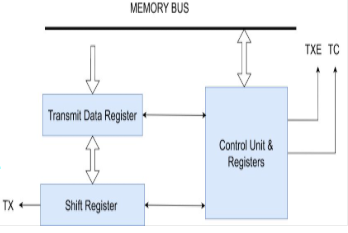
\includegraphics[width=.5\textwidth]{img/UART.png}
    \caption{UART schema logico}
    \label{img:UART_logic_scheme}
\end{figure}

Due \textbf{ISR} sono principalmente coinvolte nel processo di trasmissione:
\begin{itemize}
    \item \textbf{Transmit Empty}: indica che il contenuto del registro TDR è stato copiato nello shift register, quindi TDR può essere sovrascritto da un nuovo byte/word;
    \item \textbf{Transmit Complete}: Trasmissione completata.
\end{itemize}

Queste interruzioni vengono attivate mediante la scrittura dei registri interni della CU \textit{TXEIE} e \textit{TCE}.
Presentiamo la funzione che serve a trasmettere dati via UART in modalità interrupt \textit{IT} non bloccante. 

\begin{lstlisting}[language=C]
HAL_StatusTypeDef HAL_UART_Transmit_IT(UART_HandleTypeDef *huart, const uint8_t *pData, uint16_t Size){
  if (huart->gState == HAL_UART_STATE_READY){
   	huart->pTxBuffPtr  = pData; // Copia buffer e dimensione del buffer.
    	huart->TxXferSize  = Size;
    	huart->TxXferCount = Size;
    	huart->TxISR       = NULL;
    	huart->ErrorCode = HAL_UART_ERROR_NONE; 
    	huart->gState = HAL_UART_STATE_BUSY_TX; // Aggiorna lo stato della periferica per indicare che ci sia una trasmissione in atto.
    	// Setta la ISR da invocare in dipendenza della dimensione della parola
	if ((huart->Init.WordLength == UART_WORDLENGTH_9B) && (huart->Init.Parity == UART_PARITY_NONE))
      		huart->TxISR = UART_TxISR_16BIT;
    	else
      		huart->TxISR = UART_TxISR_8BIT;
    	/* Scatena la prima invocazione della ISR, abilitando le trasmissioni di Transmit Buffer Enable*/
    	ATOMIC_SET_BIT(huart->Instance->CR1, USART_CR1_TXEIE);
    	return HAL_OK;
  }
  else{
    return HAL_BUSY;
  }
}
\end{lstlisting}

La firma della funzione ci dice che la funzione accetta come parametri un puntatore alla struttura che contiene informazioni sulla periferica UART virtualizzata, un puntatore al buffer di dati da trasmettere, e il numero di byte da trasmettere; ritorna uno stato che può essere HAL\_OK o HAL\_BUSY. 
Se lo stato della UART è READY, allora il codice procede ad una configurazione. Presteremo particolare attenzione alla scrittura sulla CU che permette l'abilitazione dell'interruzione TXE, che è atomica.
Per poter inviare il primo carattere (oppure i primi 16 bit del messaggio, in base alla modalità) è necessario scatenare una prima interruzione di trasmissione. Per questo motivo, la funzione scrive il bit TXEIE al fine di abilitare le interruzioni nel caso di TDR vuoto. A questo punto, scatterà la prima interruzione e dato che il TDR è vuoto all'inizio, il byte/word verrà copiato in TDR e in seguito trasmesso.
Scrivere un solo bit in un registro, dato che l'architettura ARM è load-store, coinvolge almeno le operazioni di LOAD, OR e STORE. 
Supponiamo che il registro dell'unità di controllo sia a 8 bit con valore iniziale 0x00, e supponiamo che il main voglia scrivere 1 nel bit meno significativo. Se una ISR interrompe il main prima che possa fare la OR e caricare il nuovo byte sul registro, e modifica il registro per esempio scrivendo il bit più significativo, il main avrà uno stato del registro non consistente, e opererà come se la scrittura non fosse mai avvenuta. Quindi il risultato sarà determianto solo dalle istruzioni eseguite dal main (fig \ref{img:w_conflict}) 
Questa è una situazione molto diffusa durante la scrittura dei registri di controllo delle periferiche.

\begin{figure}[ht]
    \centering
    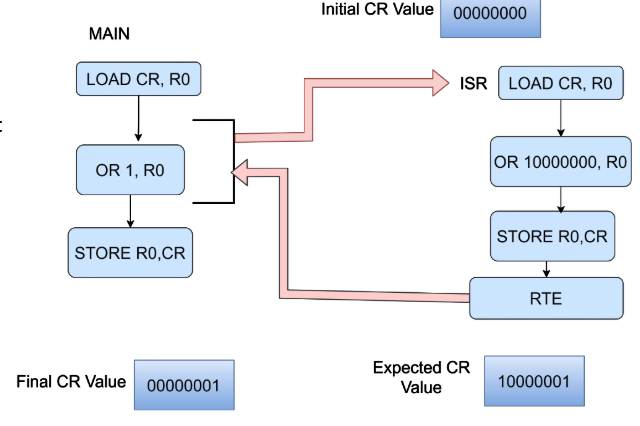
\includegraphics[width=.7\textwidth]{img/Conflitct_example.png}
    \caption{Esempio di inconsistenza}
    \label{img:w_conflict}
\end{figure}

La soluzione messa a disposizione da ARM è un \textit{TAG} esclusivo ad un determinato indirizzo di memoria, denominato \textbf{local-exclusive-monitor}. Il tag indica che l'indirizzo di memoria viene acceduto in maniera esclusiva. In particolare, ARM mette a disposizione due istruzioni per gestire i registri di memoria esclusivi:
\begin{itemize}
    \item \textbf{LDREX}: Load exclusive, carica il valore di un indirizzo di memoria ed inserisci il TAG di esclusivo;
    \item \textbf{STREX}: Scrivi il valore di un indirizzo di memoria solo se ha il tag esclusivo; Dopo la scrittura, il tag viene rimosso. Se l'indirizzo di memoria non ha il tag esclusivo, la scrittura fallisce.
\end{itemize}

Il funzionamento di questo meccanismo è illustrato dall'automa semplificato in figura \ref{img:automa_exclusive}.

\begin{figure}[ht]
    \centering
    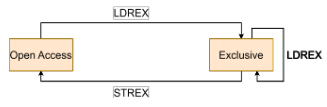
\includegraphics[width=.4\textwidth]{img/automa_exclusive.png}
    \caption{Automa semplificato}
    \label{img:automa_exclusive}
\end{figure}

Usando LDREX e STREX al posto delle normali istruzioni di LOAD e STORE, risolviamo il problema presentato precedentemente come illustrato in figura \ref{img:w_conflict_resolve}:

\begin{figure}[ht]
    \centering
    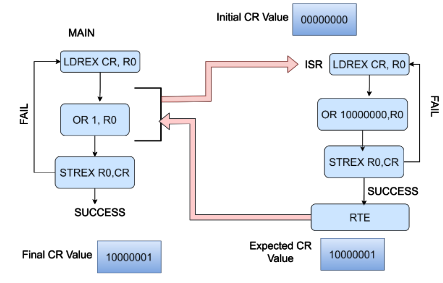
\includegraphics[width=.7\textwidth]{img/conflict_example_2.png}
    \caption{Risoluzione inconsistenza}
    \label{img:w_conflict_resolve}
\end{figure}

Questo meccanismo non causa deadlock, infatti il main riuscirà a scrivere al secondo tentativo, mentre la ISR riuscirà al primo. 
Questa funzionalità viene realizzata dalla primitiva ATOMIC\_SET\_BIT(REG,BIT):

\begin{lstlisting}[language=C]
    #define ATOMIC_SET_BIT(REG, BIT)
    do{
        uint32_t val;
        do{
            val = __LDREXW((__IO uint32_t *)&REG | (BIT));
        }while((__STREXW(val, (__IO uint32_t *)&(REG))) != 0U)
    }while(0)
\end{lstlisting}

Osserviamo che do{...}while(0) è una tecnica tipica della definizione di funzione tramite MACRO, non ha nessun significato logico a livello di codice ma solo sintattico. 


\subsection{DMA}
Nell'interfaccia grafica di CUBE \textit{Pinout \& configuration}, è possibile selezionare nell'interfaccia Connectivity le impostazioni delle varie periferiche.
Nelle impostazioni della UART, è possibile configurare le impostazioni del DMA. 
Cliccando su \textit{Request}, si può configurare il DMA il ricezione o trasmissione. Il SoC ha diversi tipi di DMA, e ogni periferica può accedere ad un determinato DMA di uno specifico tipo, non tutto è connesso a tutto. In fase di configurazione si imposta a quale DMA la periferica può accedere e in che modalità. 
L'HAL della UART offre delle funzioni per la ricezione e la trasmissione mediante DMA. Consultare l'HAL descriptor nella documentazione per ulteriori informazioni. 
